\documentclass[10pt]{article}

\usepackage[T2A]{fontenc}
\usepackage[utf8x]{inputenc}

\usepackage[russian, english]{babel}

\usepackage{vmargin}
\setpapersize{A4}
\setmarginsrb{1cm}{1cm}{1cm}{1cm}{0pt}{0pt}{0mm}{13mm}

\usepackage{amssymb, amsmath}
\usepackage{varwidth}
\usepackage{graphicx}

\sloppy

\begin{document}
	\begin{verbatim}
	...................... ........................................,-~~"""'~~-,,_
	....................... ..................................,-~"-,:::::::::::::::::::"-,
	....................... .............................,~"::::::::',::::::: :::::::::::::|',
	....................... .............................|::::::,-~"'___""~~-~"':}
	....................... .............................'|:::::|: : : : : : : : : : : : : :
	....................... .............................|:::::|: : :-~~—: : : —-: |
	....................... ............................(_"~-': : : : : : : : :
	....................... ............................."'~-,|: : : : : : ~—': : : :,'-never gonna
	....................... .................................|,: : : : : :-~~-: : ::/ —-give you up!
	....................... ............................,-"\':\: :'~,,_: : : : : _,-'
	....................... ......................__,-';;;;;\:"-,: : : :'~—~"/|
	....................... .............__,-~";;;;;;/;;;;;;;\: :\: : :____/: :',__
	....................... .,-~~~""_;;;;;;;;;;;;;;;;;;;;;;;;;',. ."-,:|:::::::|. . |;;;;"-,__
	......................./;;;;;;;;;;;;;;;;;;;;;;;;;;;;,;;;;;;;;;\. . ."|::::::::|. .,';;;;;;;;;;"-,
	.....................,' ;;;;;;;;;;;;;;;;;;;;;;;;;;;;;;|;;;;;;;;;;;\. . .\:::::,'. ./|;;;;;;;;;;;;;|
	..................,-";;;;;;;;;;;;;;;;;;;;;;;;;;;;;;;;;\;;;;;;;;;;;',: : __|. . .|;;;;;;;;;,';;|
	................,-";;;;;;;;;;;;;;;;;;;;;;;;;;;;;;;;;;;;',;;;;;;; ;;;; \. . |:::|. . .",;;;;;;;;|;;/
	.............../;;;;;;;;;;;;;;;;;;;;;;;;;;|;;;;;;;;;;;;;;\;;;;;;;; ;;;\. .|:::|. . . |;;;;;;;;|/
	............./;;,-';;;;;;;;;;;;;;;;;;;;;;,';;;;;;;;;;;;;;;;;,;;;;;;; ;;;|. .\:/. . . .|;;;;;;;;|
	............/;;;;;;;;;;;;;;;;;;;;;;;;;;,;;;;;;;;;;;;;;;;;;;;;;; ;;;;;;;",: |;|. . . . \;;;;;;;|
	.........,~";;;;;;;;;; ;;;;;;;;;;;,-";;;;;;;;;;;;;;;;;;;;;;;;;;\;;;;;;;;|.|;|. . . . .|;;;;;;;|
	.....,~";;;;;;;;;;;;;; ;;;;;;;;,-';;;;;;;;;;;;;;;;;;;;;;;;;;;;;;;;',;;;;;;| |:|. . . . |\;;;;;;;|
	....,';;;;;;;;;;;;;;;;; ;;;;;;;/;;;,-';;;;;;;;;;;;;;;;;;;;;;;;;;;;;;;,;;;;;| |:|. . . .'|;;',;;;;;|
	...|;,-';;;;;;;;;;;;;;;;;;;,-';;;,-';;;;;;;;;;;;;;;;;;;;;;;;;;;;;;;;;;,;;;;| |:|. . .,';;;;;',;;;;|_
	../;;;;;;;;;;;;;;;;;,-'_;;;;;;,';;;;;;;;;;;;;;;;;;;;;;;;;;;;;;;;;;;;|;;; ;|.|:|. . .|;;;;;;;|;;;;|""~-,
	./;;;;;;;;;;;;;;;;;;/_",;;;,';;;;;;;;;;;;;;;;;;;;;;;;;;;;;;;;;;;;;;;;;,;;| |:|. . ./;;;;;;;;|;;;|;;;;;;|-,,
	;;;;;;;;;;;;;;;;;,-'...|;;,;;;;;;;;;;;;;;;;;;;;;;;;;;;;;;;;;;;;;;;;;; ;;;;;| |:|._,-';;;;;;;;;|;;;;|;;;;;;;;
	;;;;;;;;;;;;;;,-'....,';;,;;;;;;;;;;;;;;;;;;;;;;;;;;;;;;;;;;;;;;;; ;;;;;;;;|.|:|::::"'~-~"'||;;;;;|;;;;;;;;;
	;;;;;;;;;;;;;,'....../;;;;;;;;;;;;;;;;;;;;;;;;;;;;;;;;;;;;;;;;;;;;;;;;;; ;;|.|:|::::::::::::::|;;;;;',;;;;;;
	;;;;;;;;;;,-'......,';;;;;;;;;;;;;;;;;;;;;;;;;;;;;;;;;;;;;;;;; ;;;;;;;;;;;;|:|:|::::::::::::::',;;;;;;|_""~-
	;;;;;;;;;,'......../;;;;;;;;;;;;;;;;;;;;;;;;;;;;;;;;;;;;;;;;;;;;;;;;;; ;;;;|:|:|:::::::::::::::|;;;;;;|.....
	;;;;;;;;/.......,-';;;;;;;;;;;;;;;;;;;;;;;;;;;;;;;;;;;;;;;;;;;; ;;;;;;;|:|:|:::::::::::::::|;;;;;|..........
	\end{verbatim}
	\section{Представление чисел с фиксированной точкой. Прямой, обратный и дополнительный код. Формирование битовых признаков переноса, переполнения, отрицательного результата, нуля}
	\paragraph{Представление чисел с фиксированной точкой.}
	В работе. Мне нужно перезагрузиться в другую систему, дабы найти там материалы.
	\paragraph{Прямой, обратный и дополнительный код.}
	Есть три представления чисел с фиксированной точкой в ЭВМ:
	\begin{itemize}
		\item Прямой ~--- модуль числа представляется, что для положительных, что и для отрицательных одинаково. Под знак числа отводится старший разряд. Область значений таких чисел симметрична, но ограничена тем, что у нас есть два представления нуля (положительный и отрицательный). Для N-разрядного целого двоичного числа область значений ~--- $[-2^{N-1} + 1; 2^{N-1} - 1]$;
		\item Обратный код ~--- представление положительных чисел сходно с прямым. Для представления отрицательных чисел используется инверсия положительного числа того же модуля. Для N-разрядных целых двоичных чисел область значений ~--- $[-2^{N-1}+1;2^{N-1}-1]$. Недостаток с двойным кодированием нуля также присутствует, но область значений также симметрична.
		\item Дополнительный код ~--- представление положительных чисел также как и в прямом коде. Код отрицательных чисел формируется посредством инверсии всех разрядов положительного числа и прибавлении единицы. Область значений уже не симметрична (отрицательных чисел на одно больше, если ноль считать ни тем не другим), но исправляется проблема с двойным кодированием нуля. Для N-разрядной сетки двоичных целых чисел область значений ~---$[-2^{N-1};2^{N-1}-1]$. Обоснование формулы для N-разрядных:
		\begin{align*}
			\text{Отрицательное число это:} & M' = 2^N - M,
			\text{где } & M\ge 0\\
			\text{Прибавим и вычтем из формулы 1:} & M' = 2^N - 1 + 1 - M =\\
			= ((2^N - 1) - M) + 1 &= \bar M + 1
		\end{align*}
	\end{itemize}
	\paragraph{Формирование битовых признаков результата.}
	Регистр флагов ~--- регистр процессора (FLAGS), отражающий текущее состояние процессора. Регистр флагов содержит группу флагов состояния (арифметические флаги) и флаги управления. В БЭВМ регистром состояния является регистр PS (Program State) в его младших 4 разрядах хранятся флаги NZVC.
	\begin{description}
		\item[Перенос (C)] CF (Carry Flag) ~--- арифметический флаг переноса, в нем фиксируется перенос из старшего разряда при сложении и заем в старший разряд при вычитании. При умножении CF показывает возможность (=0) и невозможность (=1) представления произведения в том же формате, что и операндов. Флаг переноса является индикатором ошибки переполнения в беззнаковой арифметике. Используется в командах ветвления (условных переходах) для беззнаковой арифметики. В БЭВМ устанавливается по результату только тогда, когда открыт вентиль SETC, для этого используются 3 сигнала (выходящие из АЛУ): $С_O$ (Carry old ~--- флаг переноса до исполнения команды), $C_N$ (Carry new ~--- новый флаг, сформировавшийся после исполнения команды), $C_{14}$ (Carry 14 ~--- перенос в 14 разряд, совсем не влияет на выставление $С$). На вход коммутатора пропускаются только 2 бита, связанные с переносом: $C_N$ (Либо как $C_N$ с АЛУ, либо как $C_O$ в зависимости от установки вентилей) и $C_{14}$, использующийся для выставления флага переполнения.
		\item[Переполнение (V)] OF (Overflow Flag) ~--- флаг переполнения. Устанавливается в командах сложения и вычитания, если результат не помещается в формате, при этом и операнды и результат интерпретируются как знаковые числа. Аппаратно он формируется совпадением переносов из двух старших разрядов при сложении и заемов в два старших разряда при вычитании (если они совпадают, то флаг равен 0). Переполнение фиксируется 3 способами:
		\begin{itemize}
			\item сравнение знаков операндов и суммы: если знак суммы отличается от знаков операндов, то фиксируется переполнение;
			\item сравнение переносов из двух старших разрядов: если они не совпадают, то фиксируется переполнение;
			\item использование модифицированного знака (под знак отводится два разряда, второй дублирует знак).
		\end{itemize}
		В БЭВМ флаг переполнения помимо того, что он выставляется лишь при открытом вентиле SETV, использует биты $C_N$ и $C_{14}$ по следующей формуле: $V = C_N \oplus C_{14}$.
		\item[Отрицательный результат (N)] SF (Sign Flag) ~--- флаг знака, в котором копируется старший разряд результата. В БЭВМ копируется именно 15 бит результата при открытом вентиле STNZ.
		\item[Флаг нуля (Z)] ZF (Zero Flag) ~--- флаг нуля, устанавливается при нулевом значении результата, в противном случае сбрасывается. В БЭВМ устанавливается с помощью 16 входового элемента ИЛИ-НЕ (NOR) при открытом вентиле STNZ.
	\end{description}
	\section{Базовые элементы вычислительной техники: ячейки, регистры, шины, вентили, тактовые генераторы, логические схемы, триггеры, счетчики, сумматоры}
	\paragraph{Ячейки}
	Для хранения информации в ЭВМ используются ячейки памяти двух видов:
	\begin{enumerate}
		\item SRAM ~--- Static Random Access Memory (Используется в основном в ПЗУ и его видах). Работает на 6 транзисторах за счет положительно-обратной связи. Не требует постоянной подзарядки, данные хранятся и без нее.
		\item DRAM ~--- Dynamic Random Access Memory (Используется в основном в ОЗУ). Требует лишь один транзистор и конденсатор (можно без если транзистор сам имеет паразитную емкость). Требует постоянной подзарядки из-за разрядки конденсатора, иначе данные теряются.
	\end{enumerate}
	\paragraph{Регистры}
	Во всех компьютерах имеются несколько регистров, доступных на уровне архитетуры набора команд. Они позволяют контролировать выполнение программы, хранить временные результаты, а также служат для некоторых других целей. Обычно регистры, доступные на уровне микроархитектуры, на уровне архитектуры набора команд недоступны, однако есть некоторые (счетчик команд, указатель стека), доступные на обоих уровнях. В то же время регистры, доступные на уровне архитектуры набора команд, всегда доступны на уровне микроархитектуры, поскольку именно там они реализованы.

	Регистры уровня архитектуры набора команд можно разделить на две категории: специальные регистры и регистры общего назначения. К специальным регистрам относятся счетчик команд и указатель стека, а также другие регистры, имеющие особые функции. Регистры общего назначения содержат ключевые локальные переменные и промежуточные результаты вычислений. Их основная функция состоит в том, чтобы обеспечить быстрый доступ к часто используемым данным (обычно без обращений к памяти). RISC-машины с высокоскоростными процессорами и (относительно) медленной памятью обычно содержат как минимум 32 регистра общего назначения, причем в новых процессорах количество регистров общего назначения постоянно растет.

	В некоторых машинах регистры общего назначения полностью симметричны и взаимозаменяемы. Если все регистры эквивалентны, для хранения промежуточного результата компилятор может использовать как регистр R1, так и регистр R25. Выбор регистра не имеет никакого значения.

	Для регистров могут существовать системные соглашения по поводу того, как нужно использовать регистры, которых разработчики компиляторов и программисты, пишущие на ассемблере, должны следовать.

	Помимо регистров, доступных на уровне архитектуры набора команд, всегда существует довольно много специальных регистров, доступных только в привилегированном режиме. Эти регистры контролируют различные блоки кэш-памяти, основную память, устройства ввода-вывода, другие устройства машины. Данные регистры используются только операционной системой, поэтому компиляторам и пользователям не обязательно знать об их существовании.

	Существует один регистр, который представляет собой <<гибрид>>, доступный и в привилегированном уровне и в пользовательском режимах. \textbf{Регистр PSW} ~--- флаговый. Содержит коды условий, устанавливаемые в АЛУ (N, Z, V, C, A, P).

	Флаговый регистр может хранить не только коды условий. Его содержимое в разных машинах может быть разным. Дополнительные поля указывают режим машины (kernel или user-space), бит трассировки, уровень приоритета процесса, статус разрешения прерываний.
	\paragraph{Шины}
	Набор проводов для передачи информации между компонентами логических схем. Имеет разрядность передаваемой информации, указанную обычно косой чертой на шине с числом разрядов рядом. На своих концах требует установку заглушек, для предотвращения отражения сигнала.
	\paragraph{Вентили}
	Один из компонентов логических схем, предназначенный для пропускания или задержки сигнала. Имеет два входа (входной сигнал и управляющий) и один выход (выходной сигнал). По сути работает как элемент И при положительном кодировании. При отсутствии управляющего сигнала (0), не пропускает сигнал на выход (0), при наличии управляющего сигнала (1) ~--- пропускает вход (1/0).
	\paragraph{Тактовые генераторы}
	Во многих цифровых схемах все зависит от порядка выполнения операций. Иногда одна операция должна предшествовать другой, иногда две операции должны происходить одновременно. Для контроля временных параметров в цифровые схемы встраиваются тактовые генераторы, позволяющие обеспечить синхронизацию. \textbf{Тактовые генератор} ~--- это схема, которая вызывает серию импульсов. Все импульсы одинаковы по длительности. Интервалы между последовательными импульсами также одинаковы. Временной интервал между началом одного импульса и началом следующего называется \textbf{временем такта}. Частота импульсов обычно составляет от 1 до 500 МГц, что соответствует времени такта от 1000 до 2 нс. Частота тактового генератора обычно контролируется кварцевым генератором, позволяющим добиться высокой точности.

	В компьютере за время одного такта может произойти множество событий. Если они должны осуществляться в определенном порядке, то такт следует разделить на подтакты. Чтобы достичь лучшего разрешения, чем у основного тактового генератора, нужно сделать ответвление от задающей линии тактового генератора и вставить схему с определенным временем задержки. Так порождается вторичный сигнал тактового генератора, сдвинутый по фазе относительно первичного.

	Связав различные события с разными перепадами (фронтами и спадами), можно достичь требуемой последовательности выполнения действий. Если в пределах одного такта нужно более четырех точек начала отсчета, можно сделать еще несколько ответвлений от задающей линии с различным временем задержки.

	В некоторых схемах важны временные интервалы, а не дискретные моменты времени. Например, некоторое событие может происходить не на фронте импульса, а в любое время, когда уровень импульса 1 высокий. Другое событие может происходить только в том случае, когда уровень импульса 2 высокий. Если необходимо более двух интервалов, нужно предоставить больше линий передачи синхронизирующих импульсов или сделать так, чтобы состояния с высоким уровнем импульса у двух тактовых генераторов частично пересекались во времени.

	Тактовые генераторы могут быть синхронными. В этом случае время существования импульса с высоким уровнем равно времени существования импульса с низким уровнем. Чтобы получить асинхронную серию импульсов, нужно сдвинуть сигнал задающего генератора,  использовав цепь задержки. Затем нужно соединить полученный сигнал с изначальным сигналом с помощью логический функции И.
	\paragraph{Защелки}
	Чтобы создать один бит памяти, нужна схема, которая каким-то образом <<запоминает>> предыдущие входные значения. Такую схему можно сконструировать из двух вентилей НЕ-ИЛИ (НЕ-И). В отличии от кобминаторной схемы, выходные сигналы защелки не определяются текущими входными сигналами.
	\paragraph{Триггеры}
	Многие схемы при необходимости выбирают значение на определенной линии в заданный момент времени и запоминают его. В такой схеме, которая называется \textbf{триггером} (flip-flop), смена состояния происходит не тогда, когда синхронизирующий сигнал равен 1, а при переходе синхронизирующего сигнала с 0 на 1 (фронт) или с 1 на 0 (спад). Следовательно, длина синхронизирующего импульса не имеет значения, поскольку переходы происходят быстро.

	Подчеркнем еще раз отличие между триггером и защелкой. Триггер запускается \textbf{перепадом сигнала}, защелка ~--- \textbf{уровнем сигнала}. Проектирование триггеров основывается на проектировании схем генерирования очень коротких импульсов и соединением их с защелками. Такие схемы основаны на том, что существуют задержки в прохождении сигналов по вентильным схемам, т. е. если один и тот же сигнал раздваивается на две линии и на обоих линиях разное число вентилей (т.е. создается задержка), которая приводит к резкому падению или скачку сигналов, что и требуется для триггеров.
	\paragraph{Счетчики}
	\paragraph{Сумматоры}
	Схема, вычисляющая бит суммы и бита переноса называется \textbf{полусумматором}. Полусумматор подходит для сложения битов нижних разрядов двух многобитовых слов. Однако он не годится для сложения битов посередине слова, потому что не может осуществлять перенос в эту позицию. Поэтому необходим \textbf{полный сумматор}, состоящий из двух полусумматоров. Имеет три входа: бит первого и второго операндов и вход переноса из предыдущего разряда. Сумматор, у которого вход переноса самого младшего бита соединен с нулем, а выход переноса ~--- со входом следующего сумматора, называется \textbf{сумматор со сквозным переносом}. В таком сумматоре сложение не закончится, пока не будет вычислен перенос для каждого разряда (что, конечно, очень медленно). Существуют более быстрые сумматоры: один из таких работает по принципу: <<разделяй и властвуй>>. Исходный сумматор разделяется на младший и два старших: таким образом, когда младший сумматор начинает сложение, старшие тоже работают (один с 0 переносом, а другой ~--- единичным), в конце, когда младший сумматор расчитал перенос для старших, из результатов двух сумматоров, выбирается тот, который вычислял по тому переносу.
	\section{Операционная система Unix ~--- ядро OC и файловая система.}
	\paragraph{Базовые понятия операционных систем}
	Операционная система ~--- является исторической заменой операторов первых ЭВМ, в чьи обязанноти входило запись программ в память ЭВМ, запуск этих программ и выгрузка из памяти результатов работы различных программ. Программы, написанные программистами, загружались в память с помощью перфокарт и считывались также на перфокарты. Современные ОС отличаются от операторов тем, что могут регулировать работу ЭВМ, выполняя несколько процессов практически одновременно, благодаря системе диспетчеризации задач. Делятся основном на 3 вида:
	\begin{enumerate}
		\item Пользовательские;
		\item Серверные или системы разделения времени ~--- буквально, эффективно разделяют процессорное время между всеми запущенными процессами;
		\item Встроенные находятся в основном в датчиках и микроконтроллерах, обслуживая физические процессы;
	\end{enumerate}
	Дополнительно выделяют системы реального времени ~--- время реагирования которых минимализируется (например, системы управления ПВО, которые должны быстро реагировать на вражеские ракеты), а также гипервизоры (Hypervisor) ~--- класс операционных систем регулирующих работу других ОС (VirtualBox, QEMU).
	\paragraph{Операционная система UNIX}
	Операционная система UNIX была разработана в компании Bell Labs в начале 70-х годов. Первая версия была написана Кеном Томпсоном (Ken Thompson) на ассемблере для мини-компьютера PDP-7. Затем появилась вторая версия для компьютера PDP-11, уже на языке C. Ее автором был Деннис Ритчи (Dennis Ritchie). В 1974 году Ритчи и Томпсон опубликовали очень важную работу о системе UNIX. За эту работу они были награждены престижной премией Тьюринга Ассоциации вычислительной техники. После публикации многие университеты попросили у Bell Labs копию UNIX. Поскольку материнская компания Bell Labs, AT\&T, была в тот момент регулируемой монополией и ей не разрешалось участвовать в компьютерном бизнесе, университеты смогли приобрести операционную систему UNIX за небольшую плату.

	Машины PDP-11 использовались практически во всех компьютерных научных отделах университетов, но операционные системы, которые  пришли туда вместе с PDP-11, не нравились ни профессорам, ни студентам. Эту нишу быстро заполнила операционная система UNIX, которая была снабжена исходными текстами, поэтому желающие могли дорабатывать ее до бесконечности.

	Одним из первых университетов, купивших UNIX, был Калифорнийский университет в Беркли. Поскольку в наличии имелись все исходные коды, в Беркли сумели существенно преобразовать UNIX. Среди изменений было перенесение этой системы на миникомпьютер VAX, создание виртуальной памяти со страничной организацией, расширение имен файлов с 14 до 255 символов, а также поддержка сетевого протокола TCP/IP, который сейчас широко используется в  Интернете (во многом благодаря тому факту, что был задействован в системе Berkeley UNIX).

	\begin{figure}[ht!]
		\centering
		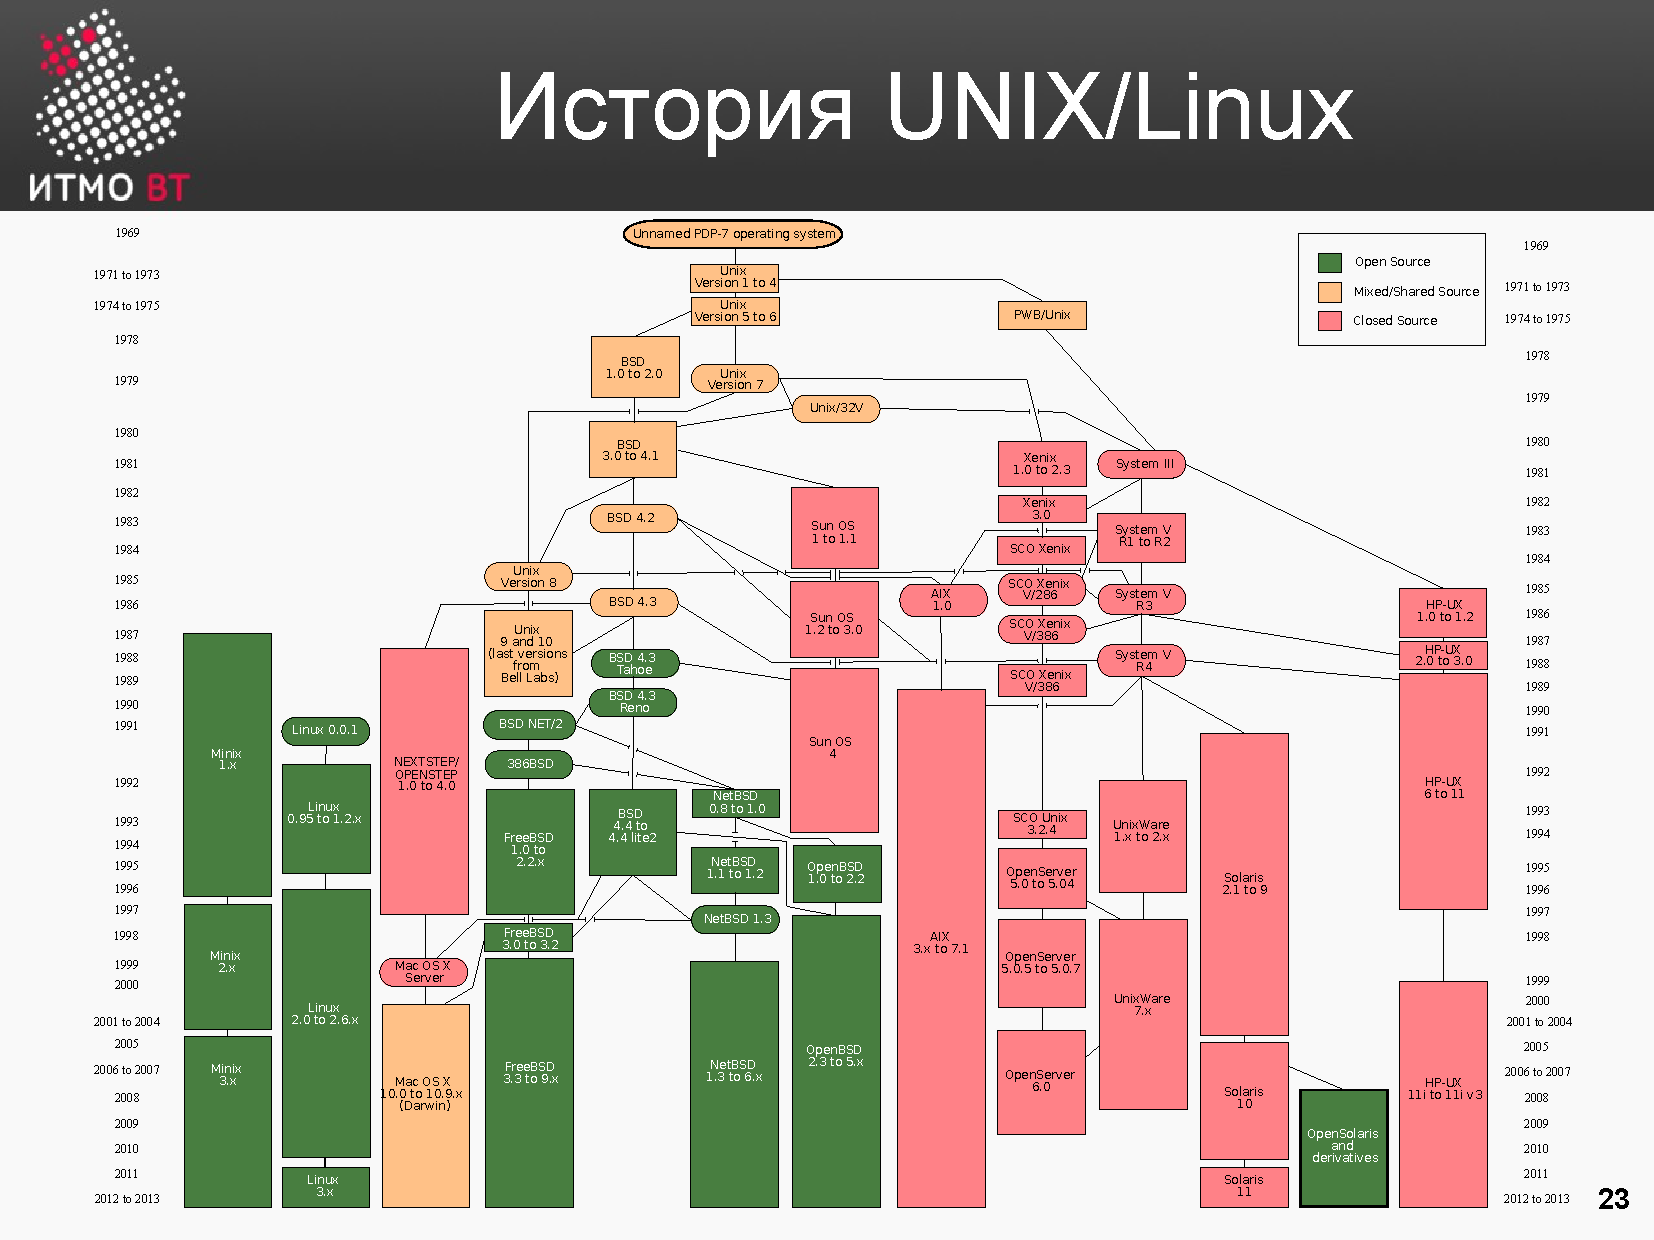
\includegraphics[width=0.9\textwidth]{assets/pages/nix_history.pdf}
	\end{figure}

	\paragraph{Интерфейс системных вызовов}
	Пока в Беркли шла вся эта работа, компания AT\&T самостоятельно продолжала совершенствовать UNIX, в результате в 1982 году появилась операционная система System III, а в 1984 ~--- System V. В конце 80-х годов широко использовались две разные и совершенно несовместимые версии UNIX: Berckeley UNIX и System V. Такое положение вещей вместе с отсутствием стандартов на форматы программ в двоичном коде в значительной степени препятствовало коммерческому успеху UNIX. Поставщики программного обеспечения не могли писать программы для UNIX, поскольку не было никакой гарантии, что эти программы смогут работать на любой версии UNIX. После долгих споров организация по стандартам в институте IEEE выпустила стандарт \textbf{POSIX} (Portable Operating System Interface) ~--- \textbf{интерфейс переносимых операционных систем}, известный также как стандарт IEEE P1003.

	Первая часть P1003.1, определяет интерфейс системных вызовов. Стандарт P1003.1 определяет около 60 системных вызовов, которые должны поддерживаться всеми системами. Это вызова для чтения и записи файлов, создания новых процессов и т.д. Сейчас практически все системы UNIX поддерживают системные вызовы, перечисленные в P1003.1, однако многие системы поддерживают и дополнительные системные вызовы, в частности те, что были реализованы в System V и в Berckeley UNIX. Обычно к набору POSIX добавляются до 200 системных вызовов.
	\paragraph{Примечание автора} К слову, минимальному набору системных вызовов достаточно содержать лишь 21 системный вызов.
	\begin{table}[h!t]
		\begin{tabular}{r | l}
			Категория             & Примеры\\\hline
			Управление файлами    & открытие или создание (open), чтение (read), запись (write),\\
			                      & закрытие (close), удаление (unlink) и блокировка файлов (fcntl)\\\hline
			Управление каталогами & каталоги по своей сути те же файлы, так что операции\\
			                      & по манипулированию файлами подходят и для каталогов\\\hline
			Управление процессами & порождение (fork), завершение (exit),\\
			                      & трассировка процессов (ptrace) и передача сигналов\\\hline
			Управление памятью    & разделение общей памяти между процессами,\\
			                      & защита страниц (subpage\_ prot)\\\hline
			Получение и установка параметров & идентификация пользователя, группы, процесса; установка приоритетов\\\hline
			Даты и периоды времени & установка времени доступа к файлам; использование\\
			                       & временных интервалов; рабочий профиль программы\\\hline
			Работа в сети & установка и выделение соединений;\\
			              & отправка и получение сообщений\\\hline
			Прочее & учет использования ресурсов; манипуляция\\
			       & дисковыми квотами; перезагрузка системы\\\hline
		\end{tabular}
	\end{table}
	\paragraph{Сетевая подсистема}
	Сфера использования сетей в большей степени относится к Berckeley UNIX, а не System V. Именно в Беркли было введено понятие \textbf{сокета} как конечной точки сетевого соединения. Моделью для этой концепции стали 4-проводные настенные розетки для телефонов. Процесс в системе UNIX может создать сокет, подключиться к нему и установить соединение с сокетом на удаленном компьютере. Через это соединение можно затем пересылать данные в обоих направлениях, обычно по протоколу TCP/IP. Поскольку сетевые технологии в системе UNIX применялись десятилетиями, значительное число серверов в Интернете используют именно UNIX.
	\paragraph{Ядро UNIX}
	Самым нижним уровнем ядра UNIX является уровень драйверов устройств, которые изолируют файловую систему от аппаратного обеспечения. Изначально каждый драйвер устройства писался без учета всех остальных и представлял собой независимую единицу, поэтому возникали дублирования, которые были практически устранены с предложения Денниса Ритчи путем ввода новой структуры \textbf{потока ввода-вывода} (stream). С помощью потоков можно установить двустороннее соединение между процессом и устройством и вставить между ними один или несколько модулей.

	\begin{figure}[ht!]
		\centering
		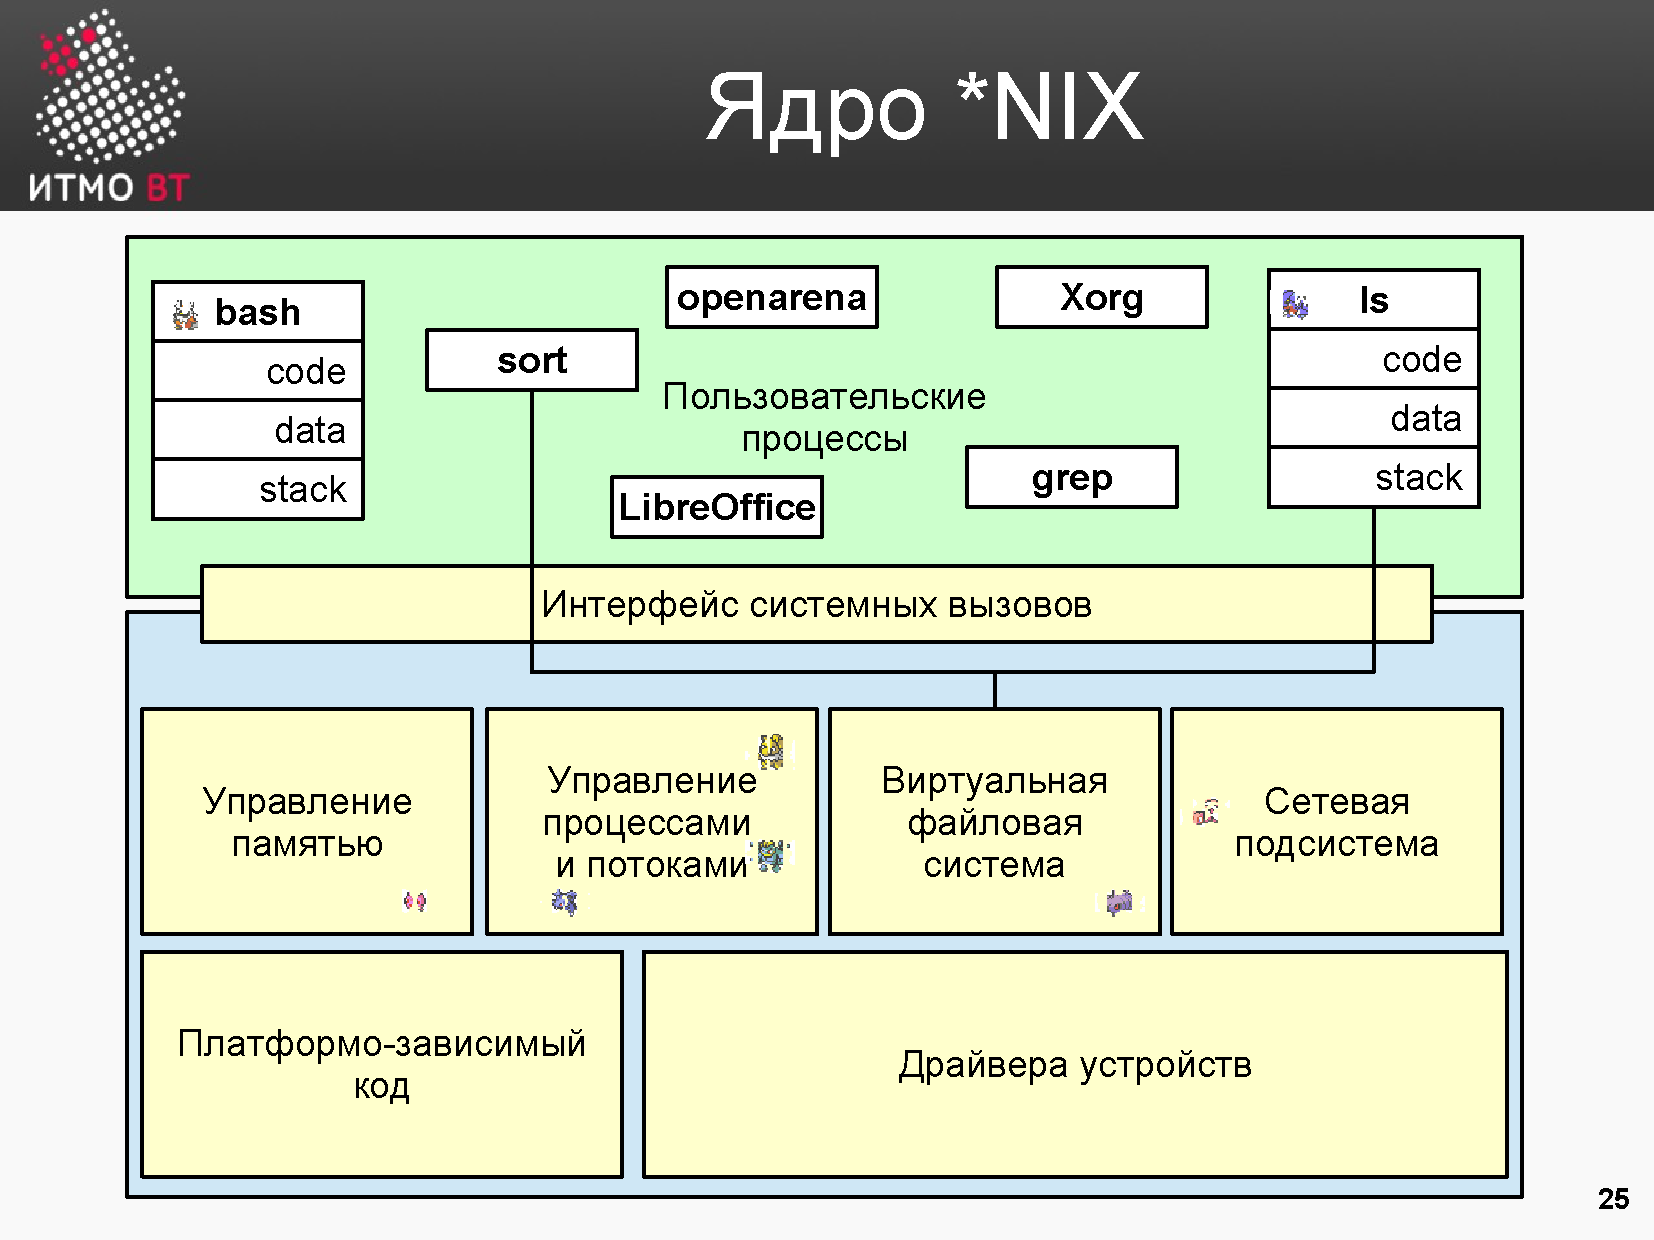
\includegraphics[width=0.9\textwidth]{assets/pages/nix_core.pdf}
	\end{figure}
	\paragraph{Управление памятью}
	Ядро имеет полный доступ к системной памяти и должны позволить процессам безопасно доступа к этой памяти, как они требуют. Часто первым шагом в этом является виртуальной адресации, обычно достигается путем подкачки и / или сегментации . Виртуальная адресация позволяет ядру сделать данный физический адрес, как представляется, еще один адрес, виртуальный адрес. Виртуальные адресные пространства могут быть различными для различных процессов; память, что один процесс обращается на определенный (виртуальный) адресе может отличаться от того, что память другого процесса получает доступ к тому же адресу. Это позволяет каждой программе вести себя так, как будто это только один (кроме ядра) работает и, таким образом, предотвращает приложения от сбоев друг друга.

	Во многих системах, виртуальный адрес программы, может ссылаться на данные, которые не в настоящее время находится в памяти. Слой косвенности обеспечивается виртуальной адресации позволяет операционной системе использовать другие хранилища данных, как жесткий диск, чтобы сохранить то, что иначе пришлось бы остаться в оперативной памяти ( RAM ). В результате, операционные системы могут позволить программам использовать больше памяти, чем система имеет физически доступна. Когда программа нуждается в данных, которая не является в настоящее время в оперативной памяти, сигналы процессора к ядру, что это произошло, и ядро отвечает записи содержимого неактивного блока памяти на диск (при необходимости) и заменить его с данными, запрошенных программа. Программа может быть возобновлено с точки, где оно было остановлено. Эта схема, как правило, известна как спрос пейджинг .

	Виртуальная адресация также позволяет создавать виртуальные разделы памяти в двух несвязанных областях, один зарезервированы для ядра ( пространства ядра ), а другие для приложений ( в пространстве пользователя ). Приложения не допускается процессором для решения памяти ядра, тем самым предотвращая приложение от повреждения работающего ядра. Этот фундаментальный раздел пространства памяти внесла большой вклад в текущие проекты реальных ядер общего назначения и является почти универсальным в таких системах, хотя некоторые исследования ядра (например, Singularity ) принимать другие подходы.
	\paragraph{Файловая система, как часть ядра}
	Над драйверами устройств находится файловая система. Она управляет файлами, каталогами, размещением дисковых блоков, защитой и выполняет многие другие функции. В системе файлов имеется так называемый \textbf{кэш блоков}, предназначенный для хранения недавно считанных с диска блоков на случай, если они понадобятся еще раз. Файловая система имеет иерархический характер, причем вершиной этой иерархии является корневой каталог, который создается при вмонтировании файловой системы (ext4, ext5, NTFS) в точки монтирования. Каждому файлу ФС сопоставляется структура \textbf{индексных дескрипторов} i-node по 64 байта, которая содержит информацию о том, кто владеет файлом, что разрешено делать с файлом, где найти данные и т.п., а также число (к слову, корневой каталог всегда имеет i-node = 2). Число выделенных i-node'ов в ФС определяет число файлов, которые можно создать. Частой практикой является невозможность создать файл, несмотря на то, что на дисковом накопителе есть свободное место (сказывается нехватка i-node'ов).

	Еще одна часть ядра системы UNIX ~--- \textbf{механизм управления процессами}. Он выполняет различные функции, в том числе поддерживает взаимодействие между процессами (InterProcess Communication, IPC) и их синхронизацию, что позволяет избежать состояния гонок. Код управления процессами также занимается планированием процессов на основе их приоритетов. Кроме того, он обрабатывает сигналы, которые представляют собой особую (асинхронную) форму программных прерываний. Наконец, он управляет памятью. Большинство систем UNIX поддерживают виртуальную память с подкачкой страниц по требованию, иногда с некоторыми дополнительными особенностями (например, несколько процессов могут совместно использовать общие области адресного пространства).

	Изначально ОС задумывалась как компактная система, благодаря чему должна была обеспечиваться надежность, производительность и отказоустойчивость. Первые версии UNIX были полностью текстовыми и ориентировались на терминалы, которые могли отображать 24 или 25 строк по 80 ASCII-символов. Пользовательским процессом управляла программа, которая называлась \textbf{оболочкой} и предоставляла интерфейс командной строки. Не является частью ядра, также как и графические интерфейсы GUI.
	\paragraph{Файловая система подробнее}
	С файловой системой тесно связана систем каталогов. Каждый пользователь может иметь несколько каталогов, а каждый каталог может содержать файлы и вложенные каталоги. Система UNIX обычно конфигурируется с главным каталогом (\textbf{корневым каталогом}), который содержит вложенные каталоги bin (для часто используемых программ), dev (для специальных файлов устройств ввода-вывода), lib (для библиотек) и usr (для пользовательских каталогов). Чтобы назвать файл, нужно указать его \textbf{путь из корневого каталога}. Путь содержит список всех каталогов от корневого каталога к файлу, для разделения каталогов используется прямой слэш.

	В каждый момент времени каждая работающая программа имеет \textbf{текущий каталог}. Путь может быть связан с текущим каталогом. Путь в котором не прописан корневой каталог называется \textbf{относительным путем}. Пользователь может создать \textbf{ жесткую ссылку} на чужой файл, использовав для этого системный вызов link. Не разрешается создавать жесткие ссылки на каталоги, чтобы предотратить циклы в системе каталогов.

	\section{Операционная система Unix ~--- интерпретаторы, стандартные потоки ввода-вывода, фильтры}
	Каждому открытому, читаемому, записываему файлу сопоставляется небольшое целое число ~--- \textbf{дескриптор файла}, которые идентифицирует его при последующих вызовах (к слову, дескрипторы 0, 1, 2 соответствуют стандартным потокам stdin, stdout и stderr соответственно). Многие программы UNIX получают входные данные из стандартного ввода и записывают входные данные в старндартный вывод, такие программы называются \textbf{фильтрами}.
	\begin{enumerate}
		\item Стандартный поток ввода ~--- файл стандартного потока ввода (stdin) имеет дескриптор 0. Из этого файла процессы извлекают свои входные данные. По умолчанию входной поток ассоциирован с клавиатурой (устройство \textit{/dev/tty}), но чаще всего он поступает по каналу от других процессов или из обычного файла.
		\item Стандартный поток вывода ~--- файл стандартного потока вывода (stdout) имеет дескриптор 1. В этот файл записываются все выходные данные процесса. По умолчанию данные выводятся на экран терминала (устройство \textit{/dev/tty}), но 
		\item Стандартный поток ошибок ~--- файл стандартного потока ошибок (stderr) имеет дескриптор 2. В этот файл записываются сообщения об ошибках, возникающих в ходе выполнения команды. По умолчанию сообщения об ошибках выводятся на экран терминала (устройство \textit{/dev/tty}), но их также можно перенаправить в файл. Зачем же для регистрации ошибок выделять специальный файл?  Дело в том, что это очень удобный способ выделения из результатов работы команды собственно выходных данных, а также хорошая возможность эффективно организовать ведение различного рода журнальных файлов.
	\end{enumerate}
	\paragraph{Интерпретаторы}
	Для обеспечения интерфейса командной строки в операционных систем часто используются командные интерпретаторы, которые могут представлять собой самостоятельные языки программирования с собственным синтаксисом и отличительными функциональными возможностями.
	В UNIX-подобных системах у пользователя есть возможность менять командный интерпретатор по умолчанию.
	С помощью интерпретатора у пользователя есть возможность давать команды операционной системе по отдельности, либо запускать скрипты, состоящие из списка команд. В первую очередь под shell понимаются POSIX-совместимые оболочки, восходящие к Bourne shell из Unix Version 7.
	Интерпретируемый язык \textit{sh} по своей сути является полноценным языком программирования. Он содержит стандартные конструкции для циклов, ветвления, объявления функций и т.п. Отличительная особенность языка \textit{sh} ~--- многие операции, которые в традиционных языках программирования являются встроенными, выполняются с помощью вызова внешних программ.
	\paragraph{Интерпретатор Bourne shell} Bourne shell является стандартным интерпретатором команд, который входит в состав всех систем UNIX и совместим с интерпретатором bash в Linux. Существуют и другие интерпретаторы, такие как bash, Korn shell (ksh) и C shell (csh).

	\section{Операционная система Unix ~--- основные команды, права файлов и способы их задания}
	С каждым файлом (а также каталогов, напоминаю, что это тоже файл) связана битовая карта, которая сообщает, кому разрешен доступ к файлу Карта содержит три поля RWX (Read, Write, eXecute) ~--- чтение, запись, выполнение). Первое из них контролирует разрешение на чтение, запись и выполнение файлов для их владельца, второе ~--- для других пользователей из группы владельца, третье ~--- для всех остальных пользователей. Включение пользователей в те или иные группы осуществляется системным администратором, которого обычно называют \textbf{привилегированным пользователем}.

	\paragraph{Основные команды}
	\begin{description}
		\item[echo] отображает на экране указанную строку текста. Не содержит stdin!
		Управляющие символы в строке:
		\begin{itemize}
			\item \textbackslash c забой строки (вроде, эмуляция backspace)
			\item \textbackslash f прогон страницы (вроде, символ новой страницы)
			\item \textbackslash n новая строка
			\item \textbackslash t горизонтальная табуляция
		\end{itemize}
		Параметры команды:
		\begin{itemize}
			\item -n запретить вывод символа новой строки (\\n)
			\item -e включить распознавание управляющих символов (аналог raw strings в python)
		\end{itemize}
		В строке можно вычислять значения переменных интерпретатора shell и даже других команд.
		\item[cat] эту команду удобно применять как для отображения содержимого файлов, так и для его создания. Из опций команды внимания заслуживает -v, активизирующая режим отображения непечатаемых символов.
		\item[pwd] эта команда отображает текущий каталог
		\item[mkdir] создание каталога
		\item[touch] создание (при отсутствии файла) или изменение времени модификации файла
		\item[ls] вывод списка файлов в директории
		\item[cd] смена текущей директории на указанную
		\item[more] постраничная распечатка stdin или файла
		\item[less] постраничная распечатка stdin или файла
		\item[cp] копирование файлов и директорий
		\item[rm] удаление файлов
		\item[rmdir] удаление пустых директорий
		\item[mv] перемещение файлов
		\item[head] вывод указанного количества строк с начала файла или stdin
		\item[tail] вывод указанного количества строк с конца файла или stdin
		\item[sort] сортировка строк файла или stdin
		\item[grep] выборка строк по шаблону
		\item[wc] подсчет количества символов, строк, слов в файле или stdin
	\end{description}
	\section{Интерфейсы ввода-вывода. Контроллеры внешних устройств. Уровни стандартизации, сопряжения с системной шиной, циклы обмена. Регистры контроллера.}
	\paragraph{Интерфейсы ввода-вывода}
	\paragraph{Что есть интерфейс?}
	\textbf{Интерфейс} ~--- <<общая граница>> между отдельными системами, через которую они взаимодействуют, совокупность средств и правил, обеспечивающих взаимодействие отдельных систем, модулями и т.п. (выдержка из википедии)

	Реализацию уже этого взаимодействия ложится на плечи программиста.
	\begin{description}
		\item[Интерфейс должен четко и однозначно определять конкретные делати обмена] (частота, набор каналов передачи, способ кодирования, команды, представления данных, набор данных и последовательность...) (примеры принципов кодирования: LE, BE; base64)
		\item[Интерфейс должен неким образом стандартизовать аппаратные и/или программная реализации]
		\item[Интерфейс должен иметь точную спецификацию и/или стандартизацию для описания способа взаимодействия] (стороны обмена должны однозначно интерпретировать детали обмена) (RFCs для TCP/IP или спецификация Java Virtual Machine)
	\end{description}
	\paragraph{Уровни стандартизации интерфейсов}
	\begin{description}
		\item[логическое подключение] (обычно некоторый набор комманд позволяющих начать или завершить подключение) (для TCP/IP, например, во время установления соединения посылаются служебные пакеты)
		\item[физические параметры сигналов] (определяет несущие части передачи) (в компьютерах в основном электрические импульсы, свет, различные виды излучения, перфокарты)
		\item[конструктивные особенности] (параметры частей позволяющих реализации интерфеса соединять между собой) (вилка-розетка)
	\end{description}
	\paragraph{Связь с интерфесов и ввода-вывода}
	Конкретная реализация системы ввода-вывода ~--- номенклатура шин в интерфейсах ввода-вывода, типы контроллеров ВУ, способы передачи информации по шинам интерфейса (параллельная или последовательная передача, синхронная или асинхронная) ~--- определяется в первую очередь назначением микроЭВМ в целом. Каким образом?

	Назначение (область применения) микроЭВМ, т.е. класс реализуемых алгоритмов, обусловливает, во-первых, выбор типа центрального процессора (векторный, скалярный или же суперскалярный) и, во-вторых, количество и перечень требуемых ВУ и каналов связи. В соответствии с этими двумя факторами в системах ввода-вывода большинства современных микроЭВМ можно выделить два уровня сопряжения ВУ с процессором и памятью. На первом уровне контроллеры ВУ сопрягаются с процессором и памятью через системный интерфейс микроЭВМ, который обеспечивает комплексирование (возможно имелось в виду, горизонтальное и вертикальное масштабирование) отдельных устройств микроЭВМ в единую систему. На втором уровне сопряжения контроллеры посредством шин связи с ВУ соединяются с соответствующими внешними устройствами микроЭВМ.
	\begin{center}
	\fbox{\begin{varwidth}{\dimexpr\textwidth-2\fboxsep-2\fboxrule\relax}\itshape
	В современных микроЭВМ можно выделить два уровня сопряжения ВУ с процессором и памятью
		\begin{enumerate}
			\item контроллеры ВУ c процессором и памятью
			\item ВУ с контроллерами ВУ
		\end{enumerate}
	\end{varwidth}}
	\end{center}

	На первом уровне сопряжения набор шин интерфейса ввода-вывода и алгоритм его функционирования полностью определяются типом БИС (Большая Интегральная Схема для тех кто уже забыл) процессора ~--- его системным интерфейсом. Несмотря на широкое разнообразие системных интерфейсов, в общем случае можно выделить два основных способа использования системного интерфейса для организации обмена информацией с ВУ:
	\begin{itemize}
		\item с применением специальных команд ввода-вывода
		\item по аналогии с обращениями к памяти
	\end{itemize}
	При подключении новых ВУ к ЭВМ возникают два вопроса о том, как устанавливается первый уровень сопряжения (КВУ с системной шиной) и как организован второй уровень сопряжения (КВУ с ВУ). Помимо этого, нужно знать: как работает КВУ по отношению к связываемым им элементам (процессору/памяти и ВУ). Сложность в том, то вся эта схема работает синхронно (нужно всегда помнить, что сигналы появляются не под нашим контролем (нет hardcodу)).
	\paragraph{Контроллеры внешних устройств}
	Во всех контроллерах в реальных реализациях выделяют дополнительные модули, отсутствующие в БЭВМ (приемо-передатчики шины данных и шины адреса) из-за относительно малого (по сравнению с современными процессорами для MIPS их 63) количества регистров и мультиплексирования одного регистра на несколько функций (сопряжение многие к одному).
	
	Обычно шины сопряжения с системной шиной имеют 3 состояния, где 3-ье ~--- состояние высокого импенданса или же проще сопротивления (ток не идет и не влияет на установленные соединения). Также присутствует логика управления, которая осуществялет передачу данных с шины, путем отключения или подключения модулей приемо-передатчиков, используя управляющие сигналы с шины. И любой контроллер содержит регистры двух типов (входные (IN) и выходные (OUT)).

	\begin{figure}[ht!]
		\centering
		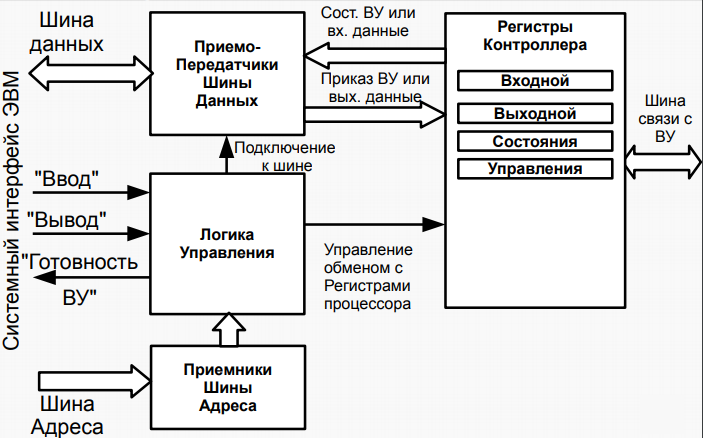
\includegraphics[width=0.5\textwidth]{assets/images/ctrlod.png}
	\end{figure}
	\paragraph{Приемопередатчики шин адреса и данных}
	Служат для физического подключения электронных схем контроллера к соответствующим шинам системного интерфейса.
	\paragraph{Логика управления}
	Выполняет селекцию адресов регистров контроллера, прием, обработку и формирование управляющих сигналов системного интерфейса, обеспечивая тем самым обмен информацией между регистрами контроллера и шиной данных системного интерфейса микроЭВМ.
	\paragraph{Сопряжение с системной шиной}
	При использовании для обмена с ВУ команд ввода-вывода адрес (номер) ВУ передается по шине адреса. Однако по этой же шине передаются и адреса ячеек памяти. Информации на шине адреса имеет смысл адреса (номера) ВУ только при наличии специальных управляющих сигналов. Такими сигналами могуть быть <<Ввод из ВУ>> <<Вывод в ВУ>>, инициируемые соответствующими командами ввода-вывода микроЭВМ.

	Для синхронизации работы процессора микроЭВМ и контроллеров ВУ а точнее, для указания моментов времени, определяющих готовность данных в ВУ для передачи либо подтверждающих их прием, может служить управляющий осведомительный сигнал <<Готовность ВУ>>.

	В любых реализациях контроллеров требуется наличие сигналов приказа на ввод <<Запись>> и вывод <<Чтение>>.
	\paragraph{Регистры контроллера}
	При разработке микропроцессора и системного интерфейса достаточно трудно предусмотреть все возможные применения ЭВМ на его основе, а следовательно, и используемые в ЭВМ ВУ. Для каждого дополнительного управляющего сигнала потребуется отдельный вывод в БИС микропроцессора. Таким образом, возникают чисто конструктивные ограничения на количество используемых в системном интерфейсе управляющих сигналов, связанных с числом выводов в БИС микропроцессора.

	Решение указанной проблемы осуществляется путем мультиплексирования шины данных, т.е. использования ее для обмена с контроллерами ВУ как данными (в одни мометны времени), так и частью управляющей информации (в другие моменты времени). Однако пересылаемая информация должна размещаться в различных регистрах контроллера ВУ: данные ~--- в регистре данных, а управляющая информация ~--- в одном или нескольких регистрах состояния и управления (количество их возрастает с увеличением сложности ВУ и уменьшением разрядности передаваемых слов, т.е. ширины шины данных). Это ставит новую задачу: выбор одного или нескольких регистров контроллера ВУ.

	Основу контроллера ВУ составляют несколько регистров, которые служат для временного хранения передаваемой информации. Каждый регистр имеет свой адрес, и зачастую такие регистры называют портами ввода-вывода. Регистры входных и выходных данных работают соответственно только в режиме чтения и только в режиме записи. Регистр состояния работает только в режиме чтения и содержит информацию о текущем состоянии ВУ (включено/выключено, готово/не готово к обмену данными и т.п.). Регистр управления работает только в режиме записи и служит для приема из микроЭВМ приказов для ВУ. В контроллерах, используемых для подключения достаточно простых ВУ, удается совместить в один регистры состояния и управления, что позволяет сократить количество используемых в контроллере портов ввода-вывода, а следовательно, и адресов, выделенных для данного ВУ.
\end{document}
